%% ------------------------------------------------------------------------- %%
\chapter{Resultados}
Apesar de todos os experimentos terem sido muito mais curtos do que inicialmente planejado, houve melhoras observadas pelo tuner. Ainda n�o foi feita a compara��o com a IA original. E tudo isso sem o OpenTuner saber como funciona o OpenTTD!

Uma observa��o � parte sobre os testes realizados: em determinado momento durante os testes no servidor R�, foi tentada uma conex�o externa com as inst�ncias de teste do jogo. O pr�prio sistema do jogo recusou a conex�o, por assumir que o cliente estava rodando em uma velocidade lenta demais para a conex�o. Isto aconteceu devido � compila��o para alta velocidade feita para o OpenTTD.

\begin{figure}[h!]\centering
	\begin{subfigure}{0.4\textwidth}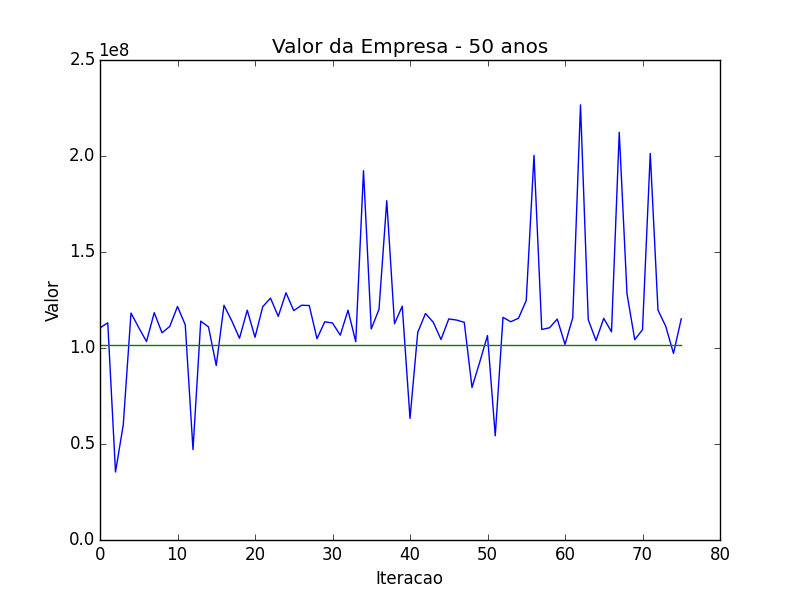
\includegraphics[width=1\linewidth]{value-50yrs}
	\end{subfigure}
	\begin{subfigure}{0.4\textwidth}
		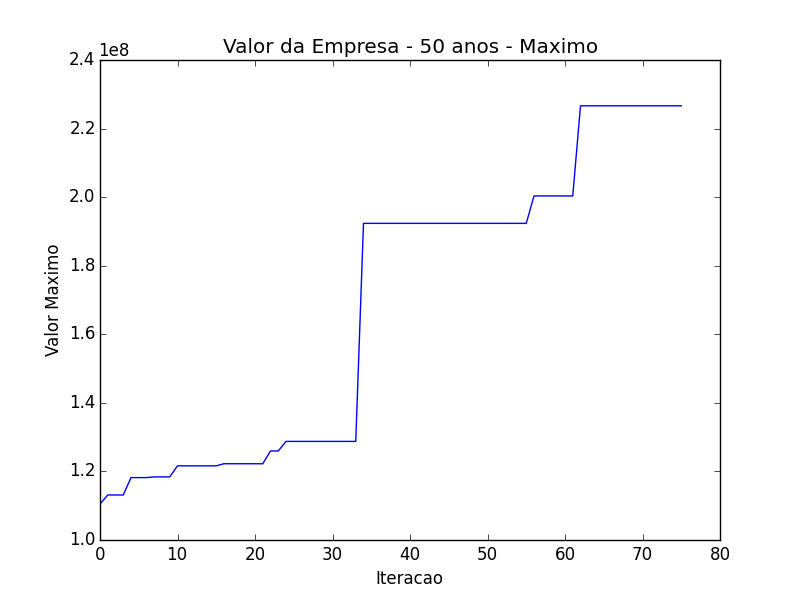
\includegraphics[width=1\linewidth]{value-50yrs-best}
	\end{subfigure}
	\caption{}
	\label{fig:value-50yrs}
\end{figure}

\begin{figure}[h!]\centering
	\begin{subfigure}{0.4\textwidth}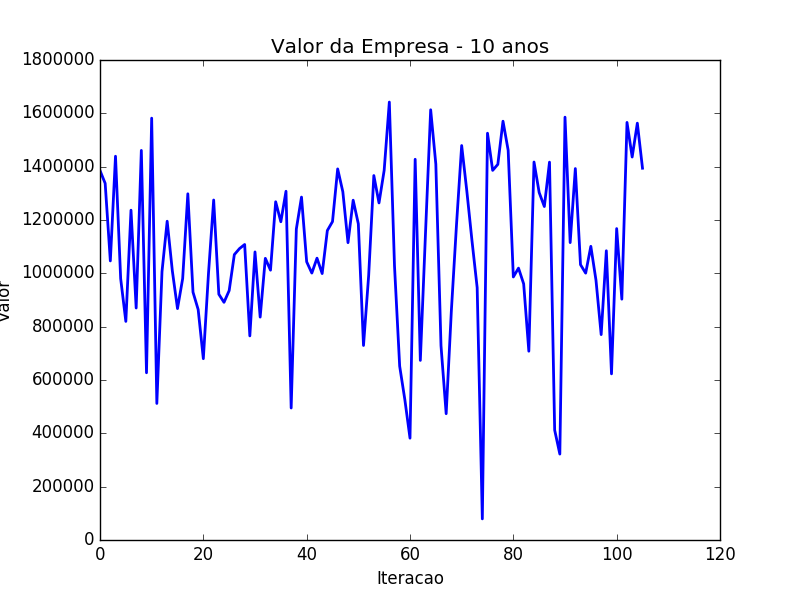
\includegraphics[width=1\linewidth]{value-10yrs}
	\end{subfigure}
	\begin{subfigure}{0.4\textwidth}
		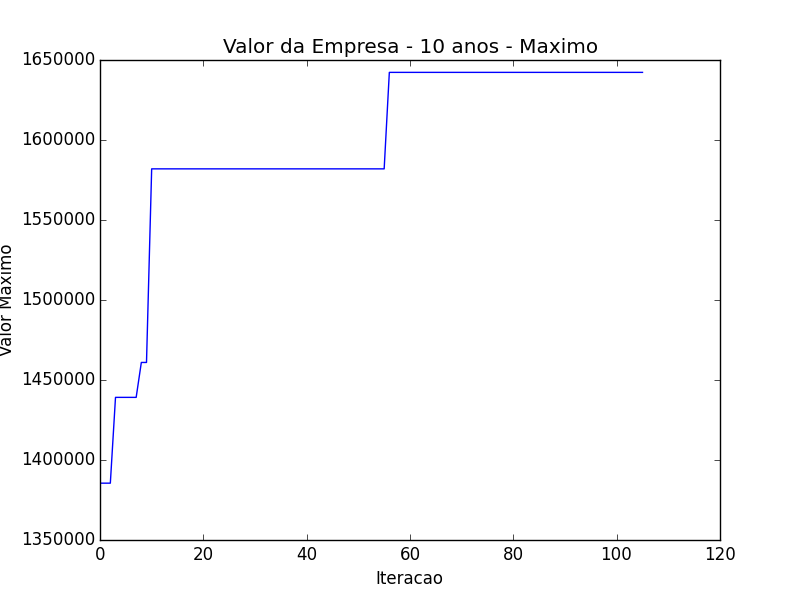
\includegraphics[width=1\linewidth]{value-10yrs-best}
	\end{subfigure}
	\caption{}
	\label{fig:value-10yrs}
\end{figure}

\begin{figure}[h!]\centering
	\begin{subfigure}{0.4\textwidth}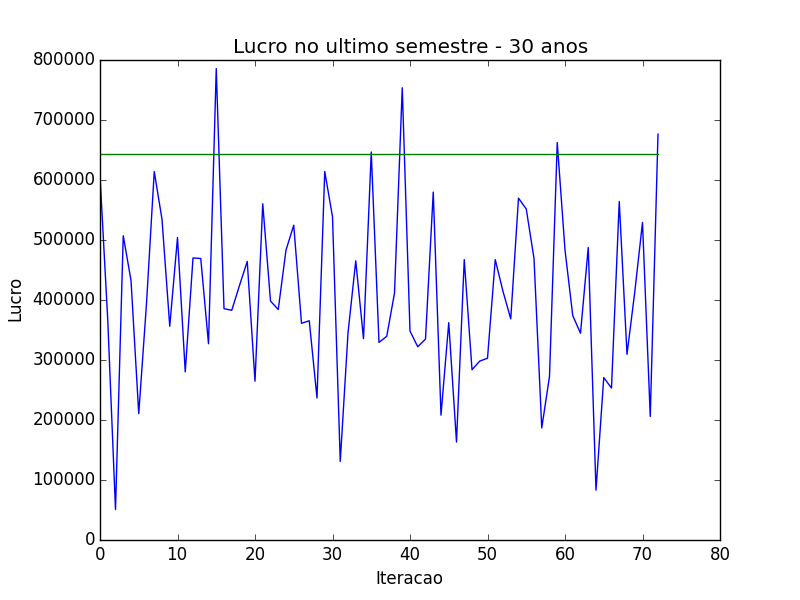
\includegraphics[width=1\linewidth]{profit-30yrs}
	\end{subfigure}
	\begin{subfigure}{0.4\textwidth}
		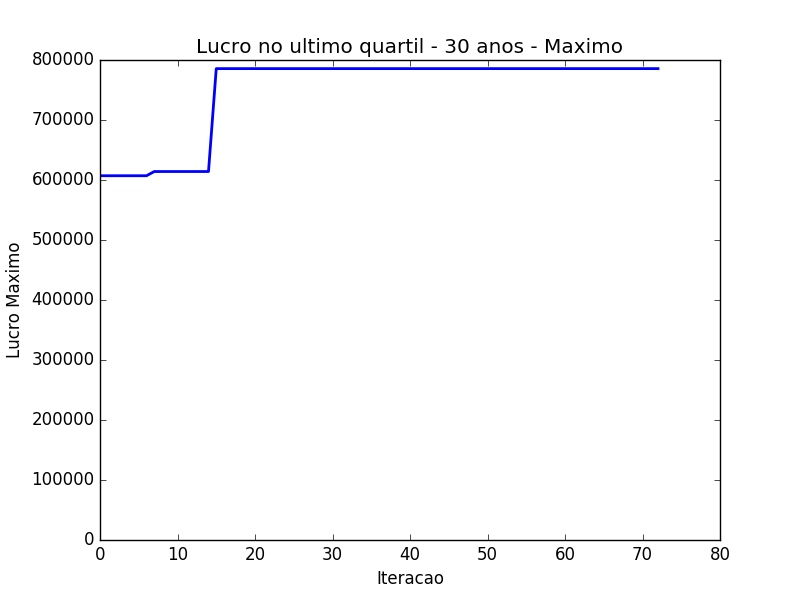
\includegraphics[width=1\linewidth]{profit-30yrs-best}
	\end{subfigure}
	\caption{}
	\label{fig:profit-30yrs}
\end{figure}

\begin{figure}[h!]\centering
	\begin{subfigure}{0.4\textwidth}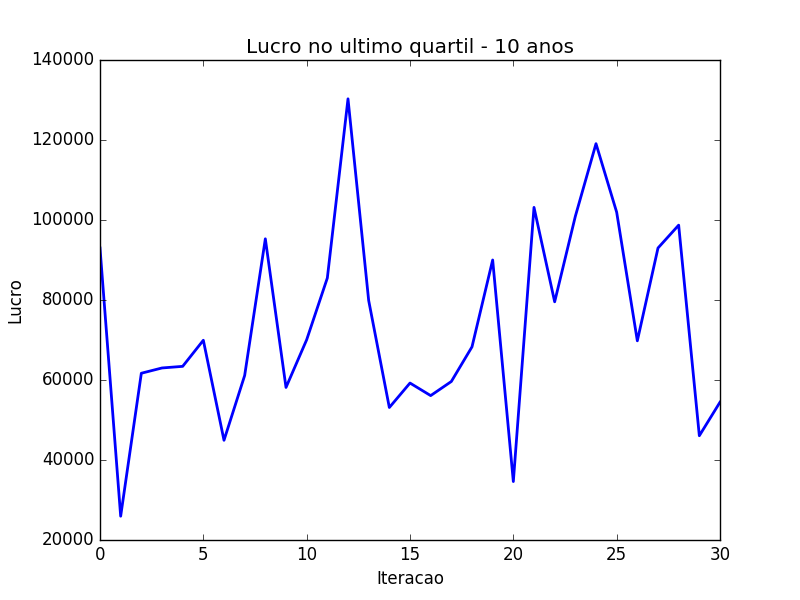
\includegraphics[width=1\linewidth]{profit-10yrs}
	\end{subfigure}
	\begin{subfigure}{0.4\textwidth}
		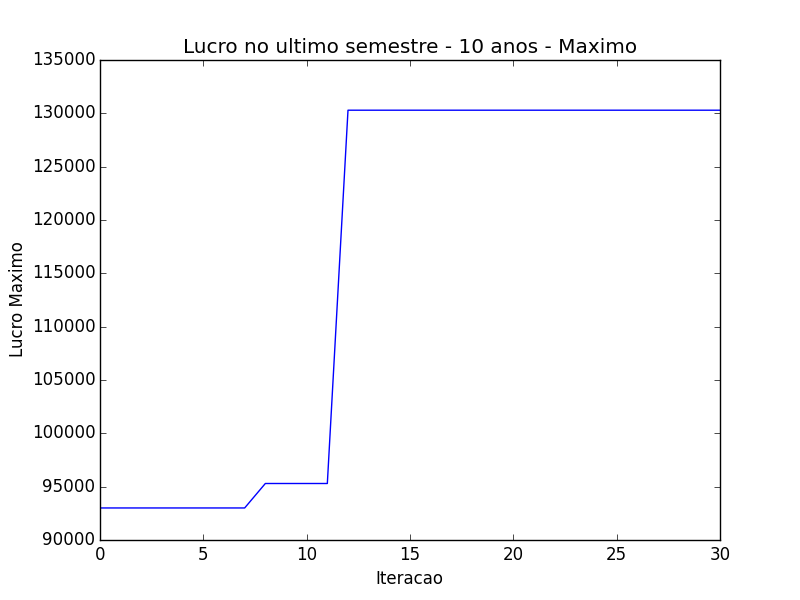
\includegraphics[width=1\linewidth]{profit-10yrs-best}
	\end{subfigure}
	\caption{}
	\label{fig:profit-10yrs}
\end{figure}

\begin{figure}[h!]\centering
	\begin{subfigure}{0.4\textwidth}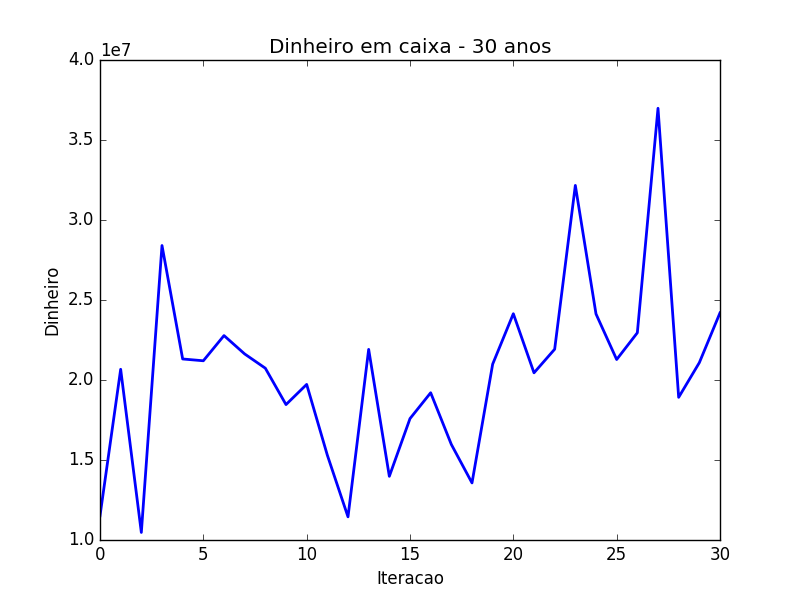
\includegraphics[width=1\linewidth]{money-30yrs}
	\end{subfigure}
	\begin{subfigure}{0.4\textwidth}
		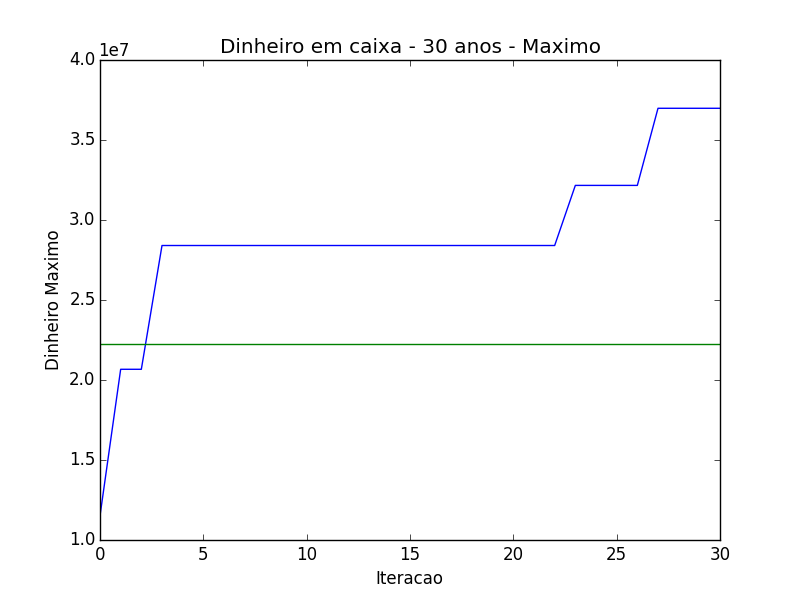
\includegraphics[width=1\linewidth]{money-30yrs-best}
	\end{subfigure}
	\caption{}
	\label{fig:money-30yrs}
\end{figure}

\begin{figure}[h!]\centering
	\begin{subfigure}{0.4\textwidth}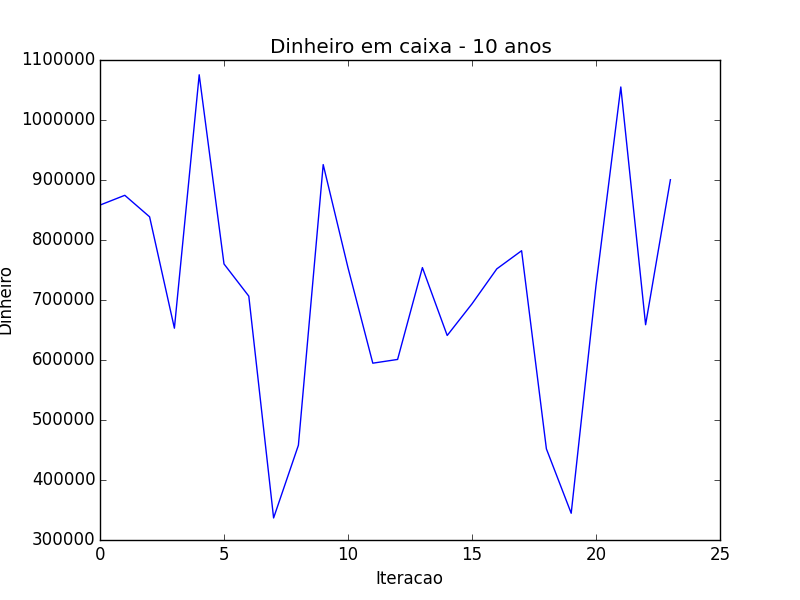
\includegraphics[width=1\linewidth]{money-10yrs}
	\end{subfigure}
	\begin{subfigure}{0.4\textwidth}
		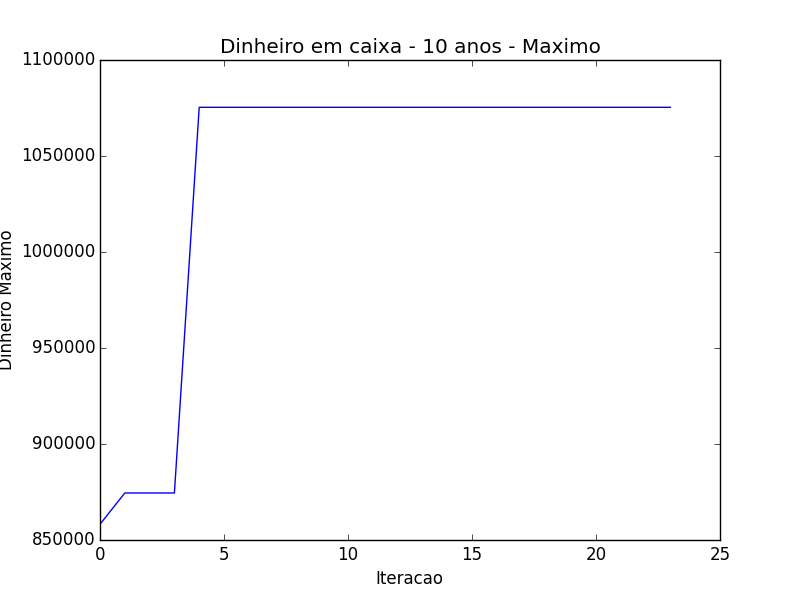
\includegraphics[width=1\linewidth]{money-10yrs-best}
	\end{subfigure}
	\caption{}
	\label{fig:money-10yrs}
\end{figure}

\chapter{Conclus�es}
\label{cap:conclusoes}

Apesar de todos os empecilhos, foi observado que o OpenTuner conseguiu melhorar os resultados observados modificando apenas o vetor de custos do algoritmo de Pathfinding usado pela IA. Mesmo esta sendo uma parte relativamente pequena de uma IA bastante complexa, e sem saber o funcionamento interno do jogo ou da IA, pode-se ver a diferen�a nos resultados obtidos. No momento, esses resultados podem ser question�veis, devido � forma como o OpenTTD lida com as IAs, j� que as medi��es podem ter tido uma vari�ncia consider�vel de tempo do jogo entre as medi��es.

Al�m disso, houve dificuldades em automatizar o OpenTTD, que n�o p�de ser compilado se simultaneamente n�o houvesse interface gr�fica e networking, exigia um conjunto de gr�ficos mesmo sendo executado em modo servidor dedicado, e compilava e carregava IAs pela primeira vez sem problemas sem suporte � biblioteca libzlo2, mas falhava ao reiniciar o jogo se fosse compilado dessa forma.
%Ser� que isso merece um bug report, se ainda n�o existir? 

Com isso em mente, talvez seja poss�vel obter resultados melhores se o jogo for desenvolvido desde o come�o para ser automatizado, e utilizando uma estrutura de \textit{tuner} que utiliza melhor as caracter�sticas do OpenTuner.
%Ali�s, se a gente for pra Rec, eu j� tenho algo em mente, mas que n�o vai dar tempo de fazer no momento.


%Provavelmente funciona yaaaaaaay mas provavelmente rende mais se o jogo for projetado assim desde o come�o yaaaaaaaaay

\chapter{Trabalhos Futuros}

Fazer um jogo com isso em mente desde o come�o pra ver � legit e se realmente ajuda no desenvolvimento de um jogo porque pode ser que n�o e eu sei l� cara aaaaaaaaaaaaaaaaaaaaaaaaaaa

%Texto texto texto texto texto texto texto texto texto texto texto texto texto
%texto texto texto texto texto texto texto texto texto texto texto texto texto
%texto texto texto texto texto texto\footnote{Exemplo de refer�ncia para p�gina
%Web: \url{www.vision.ime.usp.br/~jmena/stuff/tese-exemplo}}.

